Alun perin OAuthin kehitystyö alkoi marraskuussa 2006 kehitettäessä Twitter-pal\-ve\-luun OpenID-tukea. Pian huomattiin, ettei OpenID sovellu käytettäväksi Twitterin API-rajapintojen kanssa, vaan tarvittiin erillinen pääsynvalvontaprotokolla \cite{oauth_primer}. Siihen asti Twitter-integraatio oli toteutettu pyytämällä käyttäjää antamaan Twitter-tunnuksensa ja -salasanansa, joiden avulla palvelu integroitui käyttäjän Twitter-tiliin. Twitterin kehittämä xAuth ja siitä kehittynyt OAuth-protokolla mahdollistavat resurssien käytön ilman käyttäjätunnuksen ja salasanan luovuttamista kolmannelle osapuolelle \cite{oauth2_0}.

OAuth on määritelty RFC-dokumentissa numero 5849. Sen ensimmäinen versio (1.0) julkaistiin lokakuussa 2007 ja päivitetty versio (1.0a) kesäkuussa 2009 \cite{oauth2_0}. OAuthin versio 2.0 on myös kehitteillä ja se on tarkoitus julkaista marraskuussa 2012 \cite{oauth2_0}. OAuthin 2.0-version kehitys on ollut vaikeuksissa, lähinnä sen jatkuvasti kasvaneiden ominaisuusvaatimusten takia. Heinäkuussa 2012 pitkään protokollan parissa työskennellyt Eran Hammer jätti OAuthin 2.0 määrittelytyön, koska hänen mukaansa protokollasta on version 1.0a jälkeen peruuttamattomasti tullut liian monimutkainen, vaikeasti käytettävä ja turvaton \cite{oauth_ragequit}. OAuth 2.0 on kuitenkin käytössä useissa palveluissa, kuten Facebookissa ja GitHubissa, koska 1.0a:n ominaisuudet eivät ole riittäneet niille.

OAuth on avoin pääsynvalvontaprotokolla hajautetuille web-sovelluksille. Se mahdollistaa käyttäjien resurssien jakamisen palveluiden välillä ilman käyttäjätunnuksen tai salasanan luovuttamista kolmannelle osapuolelle. Se perustuu erilaisten valtuutusavainten välittämiseen palveluiden välillä \cite{oauth2_0}. Valtuutusavain on allekirjoitettu identiteetintarjoajalla, johon sekä käyttäjä että palvelun toteuttaja luottaa. Muun muassa Facebook tarjoaa avoimen OAuth-rajapinnan, jota web-sovellusten toteuttajat voivat käyttää pääsynvalvonnassaan.

Valtuutusavaimelle voidaan asettaa erilaisia rajoituksia esimerkiksi sen suhteen mitä tietoja käyttäjästä näytetään web-palveluun tai mihin resursseihin kyseisellä avaimella pääsee käsiksi. Kuvassa \ref{facebook_login} kirjautumisen yhteydessä Porkkanamafialle annetaan oikeus nähdä käyttäjän nimi, profiilikuva, sukupuoli jne. OAuth ei siis ole varsinaisesti tunnistautumisprotokolla, mutta valtuutusavaimen perusteella käyttäjä voidaan yksilöidä: kun käyttäjä kirjautuu myöhemmin uudestaan Porkkanamafiaan, hän hakee valtuutusavaimen Facebookilta, jota käyttämällä Porkkanamafia hakee Facebookista käyttäjän tiedot. Käyttäjän tiedoissa mukana olevalla Facebookin yksilöivällä tunnistenumerolla käyttäjä voidaan todeta samaksi kuin edellisellä kirjautumiskerralla.

Kuvassa \ref{oauth} on esitetty OAuthin käyttö, kun sitä käytetään käyttäjän tunnistamiseen. Tunnistautumispalvelin ja käyttäjähallinta voivat olla erilliset palvelut, jolloin tunnistautumispalvelin antaa pääsyvaltuuden, jonka avulla tiedot haetaan käyttäjähallinnasta (kohdat 10 ja 11). Selkeyden vuoksi tunnistautumispalvelun oletetaan toimivan myös käyttäjätietojen jakelijana.

\begin{figure}[ht]
\centering
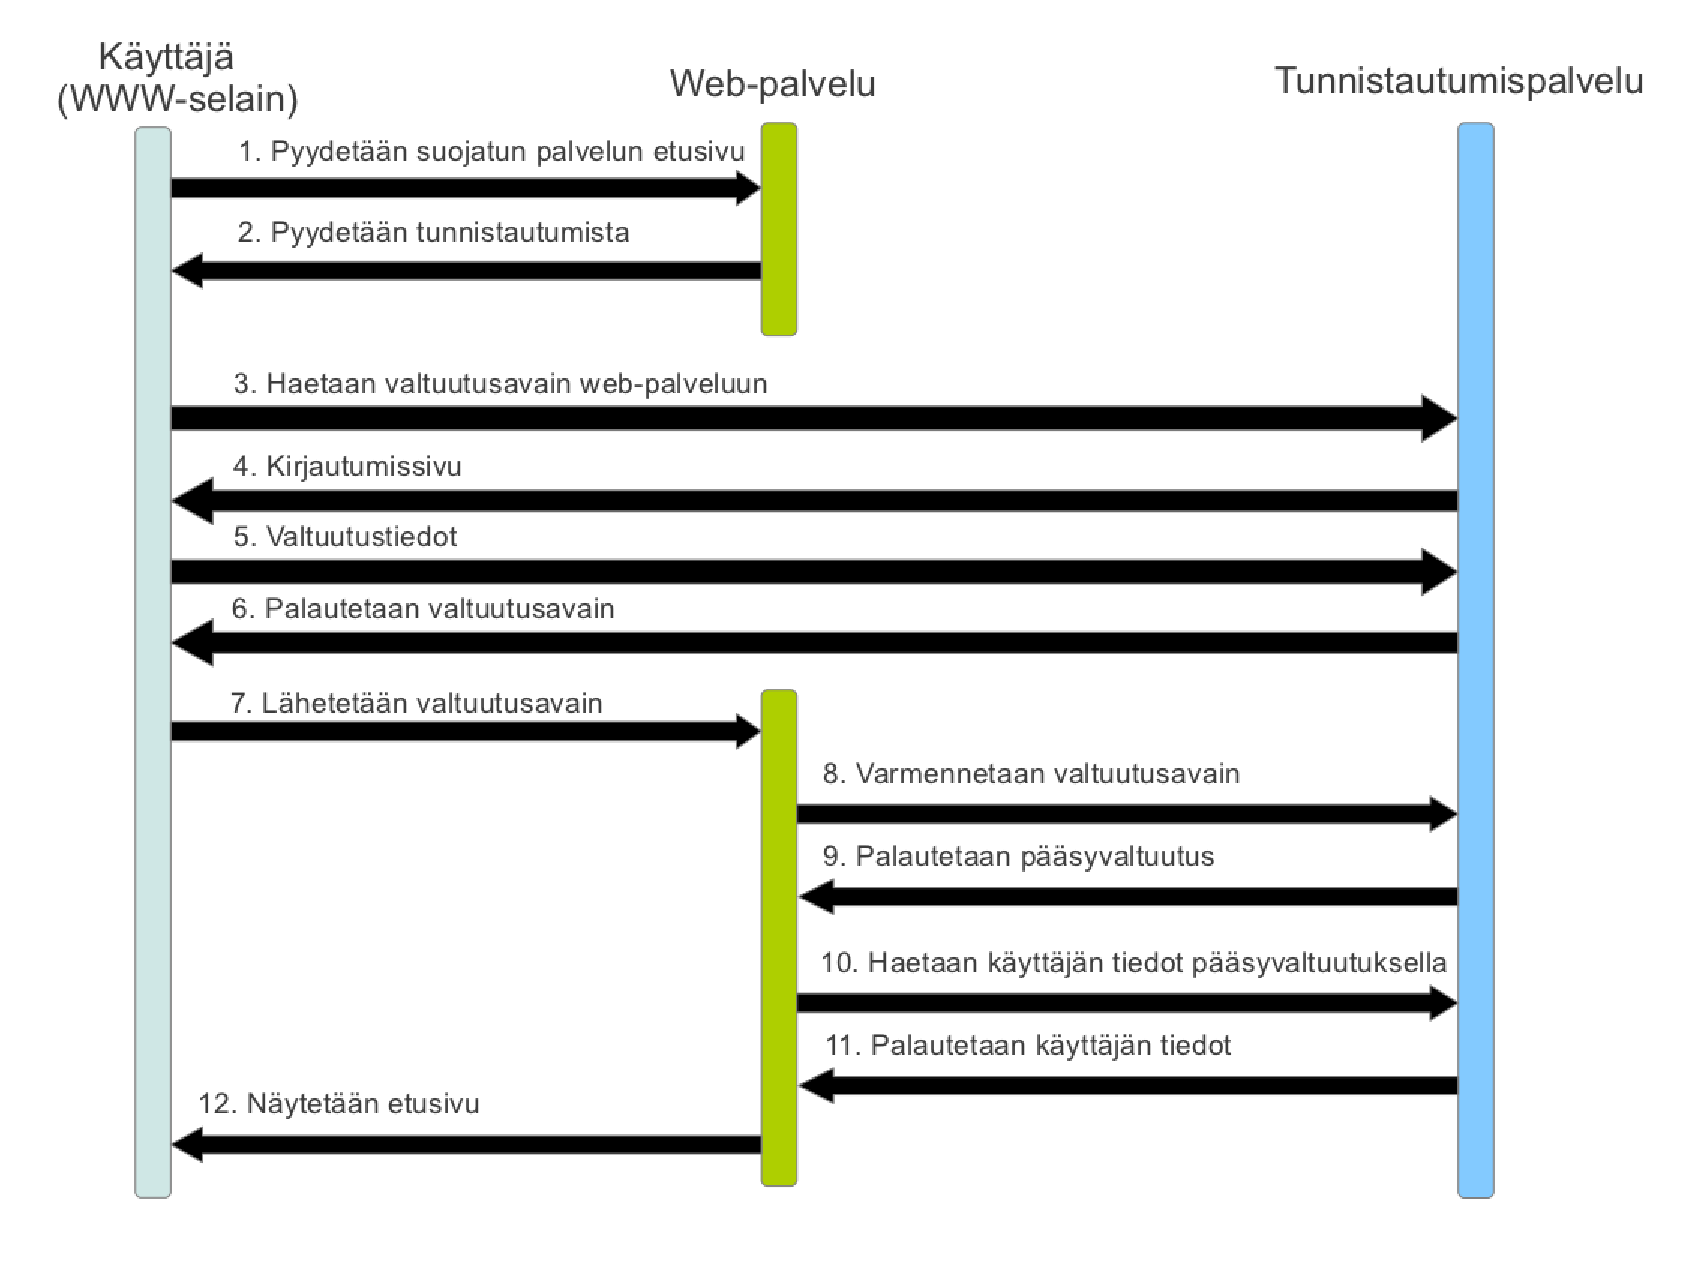
\includegraphics[width=\textwidth]{teknologiat/protokollat/oauth.eps}
\caption{OAuthin toiminta sekvenssikaaviona.}%
\label{oauth}
\end{figure}